树莓派(Raspberry Pi) (中文名为“树莓派”,简写为RPi,(或者RasPi / RPI)是为学习计算机编程教育而设计),
只有信用卡大小的微型电脑,其系统基于Linux。
随着Windows 10 IoT的发布,我们也将可以用上运行Windows的树莓派。
\par 树莓派系统镜像SD卡的内存分布图\ref{raspberryFiles}. 
\begin{lstlisting}[title=查看树莓派所属型号]
pi@raspberrypi:~ $ cat /proc/device-tree/model
Raspberry Pi 3 Model B Rev 1.2
\end{lstlisting}
\begin{figure}[htpb]
    \centering
    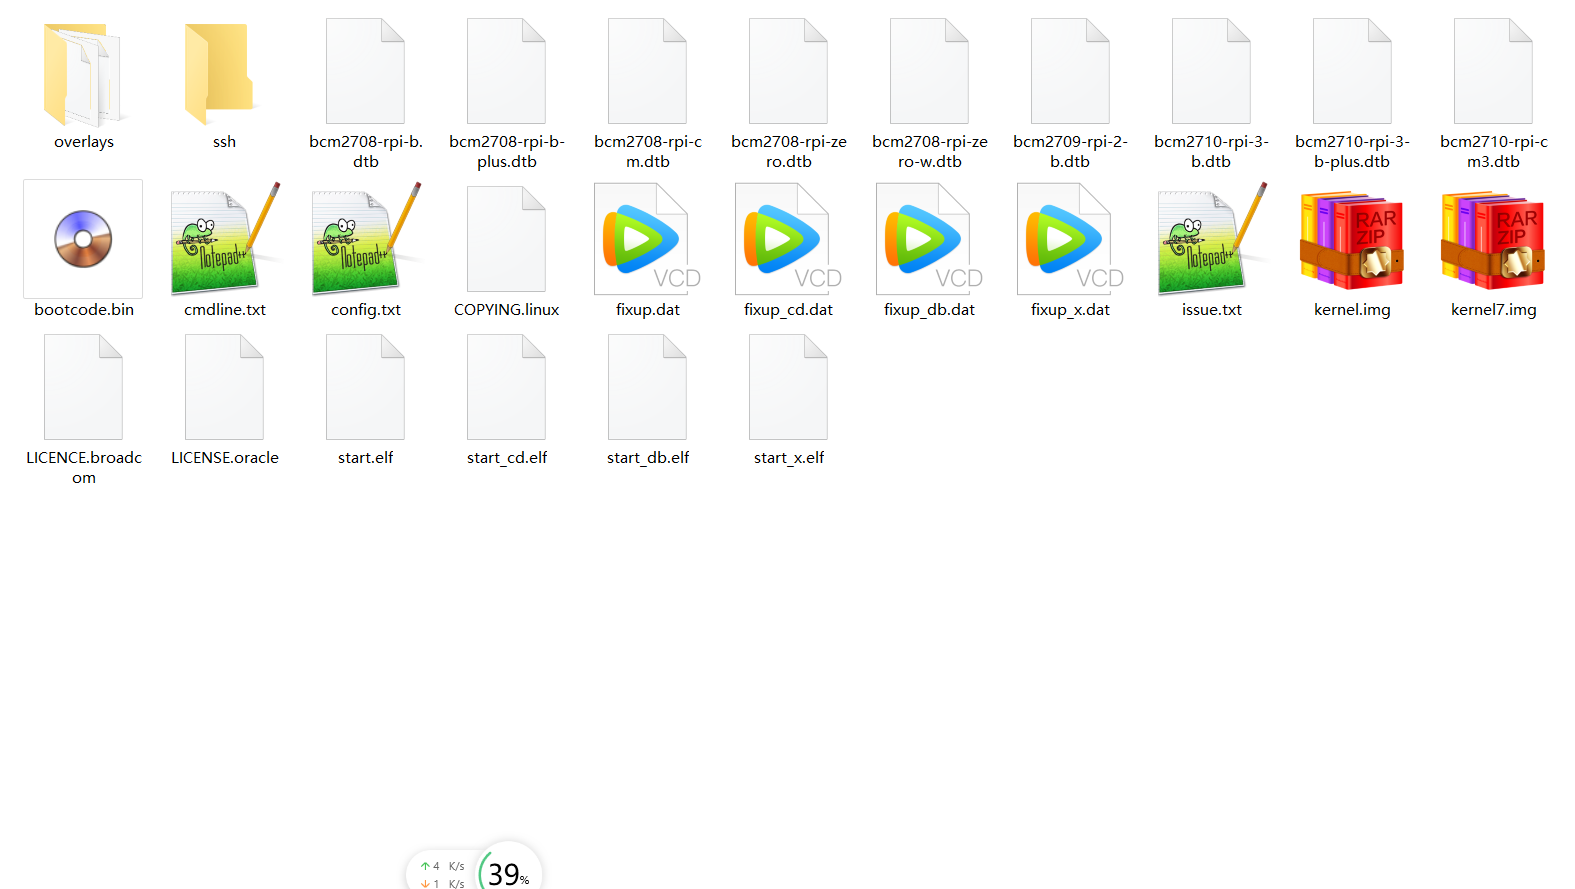
\includegraphics[width=0.8\textwidth]{pictures/raspberryFiles.png}
    \caption{Raspberry Files Structure}
    \label{raspberryFiles}
\end{figure}
其中的:
\begin{itemize}
    \item bootcode.bin: 启动文件
    \item start.elf : 类似U-Boot的BootLoader文件
    \item kernel7.img kernel.img: Linux内核文件
    \item config.txt: 配置文件
\end{itemize}
\par 对于树莓派 3B,在编译内核时,
kernel7.img 使用的是 armv7h,这可以更好的发挥处理器的性能,当然,kernel.img 也是可以用的,因为 ARM 可以向下兼容,但是无法发挥处理器的全部能力。因此在引导内核时,使用的是 kernel7.img
\par 树莓派的SoC(SoC称为系统级芯片, 片上系统)内部集成了ARM CPU,GPU,ROM,SDRAM,以及其他设备,
所以可以把树莓派想象成一股arm系统结构的PC。当给树莓派加电后,
最先执行保存在\\ROM中的代码,这些代码是芯片出厂的时候就设定的,通常被称为 first-stage bootloader,这些代码固化硬件内部,可以认为是SoC硬件的一部分。
first-stage bootloader的主要工作是加载位于SD卡上第一个分区的bootloader(称为second-stage bootloader ),第一个分区必须是FAT32格式。second-stage bootloader 主要是bootloader.bin。可以把SD卡取出,放到Windows或Linux系统中,就可以看到bootloader.bin文件。需要说明的是,上电或者重启后,cpu和ram都没有初始化,因此,执行second-stage bootloader 的实体是GPU,bootcode.bin是加载到GPU的128KB大小的L2Cache中,再执行的。bootcode.bin的主要工作是初始化ram,并把start.elf(也位于SD卡的第一分区)加载到内存中。start.elf就是third-stage bootloader,start.efl从第一个分区中加载config.txt,可以把config.txt想象成bios配置信息,内部的配置都可以改变。

\subsection{1st stage: power on}
    GPU读取ROM内容, 且运行GPU运行ROM中代码
\subsection{2nd stage: run bootcode.bin}
    GPU读取SD卡第一个FAT分区根目录下bootcode.bin
    \begin{itemize}
        \item GPU将bootcode.bin复制到L2 cache
        \item GPU执行bootcode.bin
    \end{itemize}
\subsection{3rd stage: load start.elf}
GPU读取SD卡第一个FAT分区根目录中start.elf

\begin{itemize}
    \item GPU将start.elf加载到内存中
    \item GPU开始执行start.elf
\end{itemize}
\par start.elf把ram空间划分为2部分:CPU访问空间和GPU访问空间。
SoC芯片只访问属于GPU地址空间的内存区,例如,GPU的物理内存地址空间为0x000F000 – 0x0000FFFF,
CPU的物理内存地址空间为0x00000000 – 0x0000EFFF,
如果GPU访问0x0000008,那么它访问的物理地址为0x000F008。
(实际上,ARM处理器的mmu部件把GPU的内存空间映射到0xC0000000 开始)。\par
config.txt在内存地址空间分配完成后才加载,因此,不可以在config.txt中更改内存地址的配置。
然而,可以通过配置多个elf文件来让start.elf和config.txt支持多种配置空间。
start.elf还从SD卡的第一个分区中加载cmdline.txt(如果cmdline.txt存在的话)。
该文件保存的是启动kernel(不一定是Linux的内核)的参数。至此,SoC进入了boot的最后阶段,
start.efl把kernel.img,ramdisk,dtb加载到内存的预定地址,然后
向cpu发出重启信号,因此cpu就可以从内存的预定地址执行kernel的代码,就进入了软件定义的系统启动流程。
\subsection{4th stage: load linux kernel}
GPU读取SD卡第一个FAT分区根目录中的kernel.img(Linux 内核) 到内存
\begin{itemize}
    \item 唤醒CPU
    \item CPU 开始运行kernel.img
\end{itemize}
\begin{figure}[htpb]
    \centering
    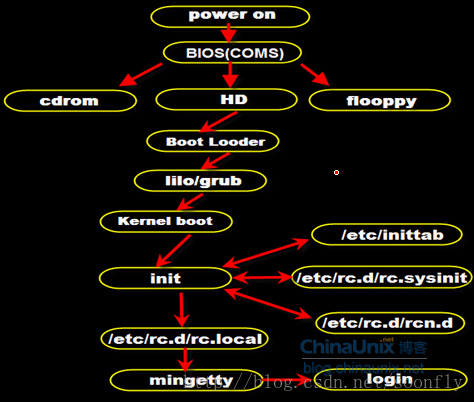
\includegraphics[width=0.9\textwidth]{pictures/raspberry_startup.png}
    \caption{linux启动流程}
    \label{rasp:startup}
\end{figure}
